\documentclass[12pt,letterpaper,noanswers]{exam}
\usepackage[usenames,dvipsnames,svgnames,table]{xcolor}
\usepackage[margin=0.9in]{geometry}
\renewcommand{\familydefault}{\sfdefault}
\usepackage{multicol}
\usepackage{wrapfig}
\pagestyle{head}
\definecolor{c03}{HTML}{FFDDDD}
\header{AM 22b Class 11}{}{Feb 22: integration}
\runningheadrule
\headrule
\usepackage{graphicx} % more modern
\usepackage{amsmath} 
\usepackage{amssymb} 
\usepackage{hyperref}
\usepackage{tcolorbox}

\usepackage[numbered,autolinebreaks,useliterate]{mcode}

\newcommand{\mb}[1]{\underline{#1}}

\begin{document}
 \pdfpageheight 11in 
  \pdfpagewidth 8.5in




% I need to review the torus trajectories...

\begin{itemize}
% \item There is a pre-class assignment (20 minutes of videos + a few WeBWorK exercises) due at 10am this Monday.  It is available on Canvas.
\itemsep0em
    % \item PSet 02 is due on Friday Feb 14th at 10am.
    \item Problem set 03 is due on Thursday Feb 25th at 6pm.
    \item There is a skill check in class today (C08, C09, C10).  The next skill check is on Friday (C11, C12).
\end{itemize}

\hrule
\vspace{0.2cm}

% partial derivatives, gradient
% local linearity, differential, directional deriv
% 2nd order partials + equations with partials

\noindent\textbf{Big picture}

This week we are studying integration for functions of multiple variables.  Today our focus is on the Riemann sum and on using the iteration of integrals from single-variable calculus to compute the integral of a function of multiple variables.

\vspace{0.2cm}
\hrule
\vspace{0.2cm}
\noindent\textbf{Skill Check C11 Practice}

\begin{questions}
\item Let $D$ be the unit disk centered about the origin in $xy$-space.  Identify the sign of $\int_D xy\ dA$.
\begin{oneparcheckboxes}
\choice positive
\choice zero
\choice negative
\end{oneparcheckboxes}

\emph{See the beginning of the problems section in \S 16.1 for about sixteen more examples (odd numbered problems have answers at the end of the text).}
\end{questions}

\vspace{0.2cm}
\hrule
\vspace{0.2cm}

\noindent\textbf{Skill Check C11 Solution}
$xy$ will be positive in the first and third quadrants.  It will be negative in the second an fourth quadrants.  For every small box $\Delta A$ in the first quadrant (containing the point $(a,b)$), there is a corresponding small box in the second quadrant (containing point $(a,-b)$).  We have $f(a,b) = -f(a,-b)$, and the contribution of those two small boxes to the integral is equal and opposite.  We can make the same argument for the contributions of the third and fourth quadrants.

The integral will be zero due to this symmetry.




\vspace{0.2cm}
\hrule
\vspace{0.2cm}


% Example: wealth and income.  one is the integral of the other (approximately).  which way?

% mean temperature of the planet

% discounting requires an integral.

% any kind of weighting function will be a sum / integral

% averaging: take a running tally.  you're invoking the notion of an integral.  go back and forth between the discrete and continuous notions of an integral.

% food intake and weight gain.

% GDP.  GDP per capita vs for the country is a spatial average.  compare communities.  need a distribution function of GDP spatially and temporally.

% population: in the US the census is setting the discretization boxes for demographic data.



% Chain rule motivation: if there is a nonuniform pollutant field and a nonuniform temperature field, and I was moving.  What would I feel as a function of time?  I will experience it as a change in time but the change is a consequence of me moving through space.  There is a linear variation in temperature from the bottom of the grand canyon to the top.  Grab one of the temperature textbook problems.  Wrote a paper with Samuel... you think things are changing in time but its because you are moving.  Worms thermotax.
% grab an image from the paper.  fig 5cd. https://www.seas.harvard.edu/softmat/downloads/2006-12.pdf

% examples for triple integrals: 
% if an organism is moving through a liquid, and whatever is in the liquid is degrading and the organism samples over time, the organism sees an average value of the concentration (senses an average value).  Can they convert that word problem into an integral?  get rid of the path integral by sampling... $\phi$ is a function of time... average over all possible paths.  Blur the path integral and replace it with.


% can i look up some kind of simple volcanic island growth model.


\noindent\textbf{Teams}

You will work with this team on the in-class problems today.  Share with your group something you like (or dislike) about winter weather.
\begin{multicols}{2}
1.  students here


\end{multicols}

%\vspace{0.2cm}
\hrule
\vspace{0.2cm}
\noindent\textbf{Single variable example: sign of an integral}

Let $C$ be the region of the $x$-axis such that $-1\leq x \leq 1$.  By convention, $\int_C 1\ dx$ is positive (i.e. this notation indicates that the interval $C$ is being traversed in a `positive' direction).  Without calculating the integral, find the signs of
   $\displaystyle\int_C dx$,
    $\displaystyle\int_C x\ dx$,
   $\displaystyle\int_C (x-1)\ dx$. %\emph{pollQ}
   
   \vspace{1.5in}

\vspace{0.2cm}
\hrule
\vspace{0.2cm}

\begin{tabular}{|c|c|c|c|}
\hline
domain dimension & integral & Riemann sum & domain (cut in pieces)  \\
\hline
$f(x)$, 1d. & $\displaystyle\int_C f(x)\ dx$ & $\displaystyle\sum\limits_{i}f(x_{i})\Delta x$ & 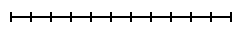
\includegraphics[scale=0.7]{img/C11line.png}    \\
\hline
$f(x,y)$.  2d. & $\displaystyle\int_R f(x,y)\ dA$ & $\displaystyle\sum\limits_{i}f(x_{i},y_i)\Delta A$ &  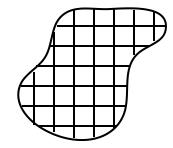
\includegraphics[scale=0.7]{img/C11region.png}   \\
\hline
\end{tabular}

\vspace{0.2cm}
\hrule
\vspace{0.2cm}


\noindent\textbf{Integration: functions of multiple variables} \S 16.1
\begin{tcolorbox}
\begin{itemize}
\item The \textbf{indefinite integral} is not easy to generalize to functions of multiple variables.
\item A \textbf{definite integral}, $\int_C f(x)dx$, is defined in terms of a limit of Riemann sums.  We can generalize this definition.  
\item Let $f:\mathbb{R}^2\rightarrow \mathbb{R}$.  Cut the region $R$ into small rectangles of size $\Delta A$.  The sum $\displaystyle\sum\limits_{i}f(x_{i},y_i)\Delta A$, where $i$ indexes the rectangles and $(x_i,y_i)$ is a point chosen from rectangle $i$, is called a \textbf{Riemann sum}, and is an approximation of the integral $\displaystyle\int_{R} f(x,y) dA$.
\item Let $f:\mathbb{R}^3\rightarrow \mathbb{R}$.  Cut the region $W$ into small rectangular prisms of size $\Delta V$.  The sum $\displaystyle\sum\limits_{i}f(x_{i},y_i,z_i)\Delta V$, where $i$ indexes the prisms and $(x_i,y_i,z_i)$ is a point chosen from prism $i$, is called a \textbf{Riemann sum}, and is an approximation of the integral $\displaystyle\int_{W} f(x,y,z) dV$.
\end{itemize}
\end{tcolorbox}





\noindent\textbf{Example (mass)}  Assume the figure below shows the density of an object in kilograms per meter squared.  The $x$- and $y$-axes are measured in meters.

Find an estimate for the mass of the object.  %\emph{pollQ}
\begin{center}
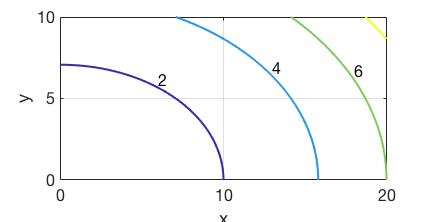
\includegraphics[width=2.5in]{img/C17p3.png}
\end{center}
\vspace{0.5cm}

\vspace{1.5in}


% \noindent\textbf{Example (mean value).} Assume the mass of the object is $400$ kilograms.  If it were, find the mean density of the object in kilograms per meter squared.
% \vspace{0.5cm}

% \vfill




% \vfill

% \noindent\textbf{Example (sign of an integral - two variables).}  
% Let $R$ be the unit disk in $\mathbb{R}^2$ (the $xy$-plane).  Without calculating the integral, find the signs of
% \begin{center}
% $\displaystyle\int_R dA$, $\displaystyle\int_R x\ dA$, $\displaystyle\int_R e^{xy}\ dA$.  \emph{pollQ}\end{center} 


% \vfill


% \begin{tcolorbox}
% \textbf{For your reference (section 16.1)}:
% Suppose the function $f$ is continuous on $R$, the rectangle $a\leq x\leq b, c\leq y \leq d$.  Cut $R$ into subrectangles of size $\Delta A$.  If $(u_{ij},v_{ij})$ is a point in the $ij$-th subrectangle, we define the \emph{definite integral} of $f$ over $R$
% $\displaystyle \int_R f\ dA = \lim\limits_{\Delta A\rightarrow 0 } \sum\limits_{i,j}f(u_{ij},v_{ij})\Delta A$. \\

% The sum $\sum\limits_{i,j}f(u_{ij},v_{ij})\Delta A$ is called a \emph{Riemann sum}. (Riemann did this work around 1854.  Published in 1867, after his death. \href{https://books.google.com/books?id=4JprCQAAQBAJ&pg=PA221&dq=riemann+sum+history&hl=en&sa=X&ved=0ahUKEwijlaKLgYbeAhVpk-AKHTHdCUkQ6AEIKTAA#v=onepage&q=riemann%20sum&f=false}{\color{blue}(Weblink to ``Elements of the History of Mathematics'')}) \\

% Let $x, y, f(x,y)$ all represent lengths, with $f$ positive.  $\int_R f\ dA$ is the \emph{volume} under the graph of $f$ above the region $R$.  \\

% Let $x, y$ represent lengths.  $\int_R 1\ dA = \int_R dA$ is the \emph{area} of the region $R$.  (The $1$ is unitless). \\

% The \emph{mean value} of $f$ on the region $R$ is $\displaystyle \frac{1}{\text{Area}(R)}\int_R f \ dA.$
% \end{tcolorbox}
% % \vspace{1cm}

% \eject


% \begin{multicols}{2}
% \noindent\textbf{Example (volume).} The solid below $f(x,y) = 3+x - \frac{y}{2}$ and above the region $R$ where $x^2+y^2\leq 1$ in the $xy$-plane has volume $\displaystyle\int_R(3+x- \frac{y}{2})\ dA.$

% \hfill\includegraphics[width=2in]{img/C17p5-18.png}
% \end{multicols}




\noindent\textbf{Volume} Assuming $x$, $y$, and $f(x,y)>0$ each indicate a distance, the solid below $f(x,y)$ and above the region $R$ in the $xy$-plane has volume $\displaystyle\int_R f(x,y)\ dA.$. The mean height of $f(x,y)$ on the region $R$ is $\frac{1}{\text{size}(R)}\int_R f(x,y)dA$. Similarly, $\displaystyle\int_C f(x)\ dx$ is an area for $f(x)>0$ and the mean height of $f(x)$ on the region $C$ is $\frac{1}{\text{size}(C)}\int_C f(x,y)dx$.
\vfill


\noindent\textbf{Area} Assuming $x$, $y$ each indicate a distance, the region $R$ in the $xy$-plane has area $\displaystyle\int_R 1\ dA.$ (where $1$ is dimensionless in this calculation).  Similarly, $\displaystyle\int_C 1\ dx$ is the length of region $C$.
\vfill

%\includegraphics[width=3in]{img/C17p5.pdf}
%\includegraphics[width=4in]{img/C17p7-18.png}

\noindent\textbf{Sign of an integral}.  By convention $\int_R dA$ is positive.  

Let $D$ be the region inside the unit circle centered at the origin.  Let $B$ be the bottom half of that region. Is $\int_D (y-y^3)\ dA$ positive, negative, or zero?  
Is $\int_B (y-y^3)\ dA$?
\vspace{1in}


\noindent\textbf{Computing double integrals via iterated integrals}:  \S 16.2
\begin{tcolorbox}
\begin{itemize}
\itemsep0em
    \item We'd like to use our knowledge of integration from single variable calculus to compute integrals over higher dimensional domains.  
    \item For Riemann sums: $\displaystyle\sum\limits_{i}f(x_{i},y_i)\Delta A$.  Write $\Delta A = \Delta x \Delta y$.  $\displaystyle\sum\limits_{i}f(x_{i},y_i)\Delta x\Delta y$.  Now change our box indexing: label a box in $R$ as the $i$th box in the $x$-direction and the $j$th in the $y$-direction, so our Riemann sum becomes $\displaystyle\sum\limits_{i,j}f(x_{i,j},y_{i,j})\Delta x\Delta y$.
    \item Sum the function along the $x$-direction first, then along the $y$: $\displaystyle\sum\limits_{i,j}f(x_{i,j},y_{i,j})\Delta x\Delta y = \displaystyle\sum\limits_{j}\left(\sum\limits_{i}f(x_{i,j},y_{i,j})\Delta x\right)\Delta y$.
    \item  $\displaystyle\int_{y=a}^{y=b}\left(\int_{x=g_1(y)}^{x=g_2(y)}f(x,y)\ dx \right)\ dy = \int_{a}^{b}\int_{g_1(y)}^{g_2(y)}f(x,y)\ dx \ dy$, after taking the limits to turn these sums into integrals.
    \item The bounds above mean that the shape of $R$ extends from $g_1(y)$ on the left to $g_2(y)$ on the right.  It's projection onto the $y$-axis is the line $a\leq y \leq b$.
    \item The \textbf{limits of the outer integral} never depend on the variables on integration.
    \item The order of integration (for the integrals we'll do in this class) can be exchanged. $\displaystyle\int_{y=c}^{y=d}\left(\int_{x=a}^{x=b}f(x,y)\ dx\right)\ dy = \int_{x=a}^{x=b}\left(\int_{y=c}^{y=d}f(x,y)\ dy\right)\ dx$ (see \textbf{Fubini's theorem} for conditions, 1907).
\end{itemize}
\end{tcolorbox}


% \noindent\textbf{Example (iterated integrals).} For a function of one variable, $\int_C f\ dx$ over a region $C$ where $a\leq x \leq b$ can be computed via the definite integral $\int_a^b f\ dx$.  By convention, $\int_C f\ dx$ always denotes that the integral is taken from the left to the right.

% For a function of two variables, $\int_R f\ dA$ is usually computed one of two ways:\begin{itemize}
%     \item (horizontal strips) integrating first in $x$ and then integration the result in $y$
%     \item integration first in $y$ and then integration the result in $x$
% \end{itemize}
% By convention, $\int_R f\ dA$ always denotes that the integral is taking from left to right in $x$ and from bottom to top in $y$.

% 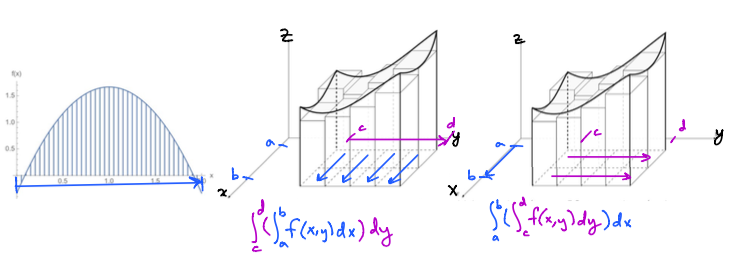
\includegraphics[width=\linewidth]{img/C17p8-18.png}
% \vfill

\noindent\textbf{Example (triangular region).}  Set up an iterated integral for $\int_R f\ dA$ where $f$ is an unknown function of two variables and $R$ is the triangular region shown below.

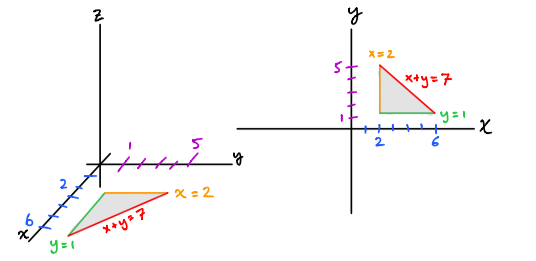
\includegraphics[width=3.5in]{img/C17p9-18.png}

\vfill

\noindent\textbf{Example (triangular region).}  For $R$ above, we'll use iterated integrals to compute $\int_R (xy)\ dA$.

\vfill




\noindent\textbf{Example (half-disk region).}  Set up an iterated integral for $\int_R x\ dA$ where $f$ is as given in the integral, and $R$ is the half-disk shown below. %\emph{pollQ}

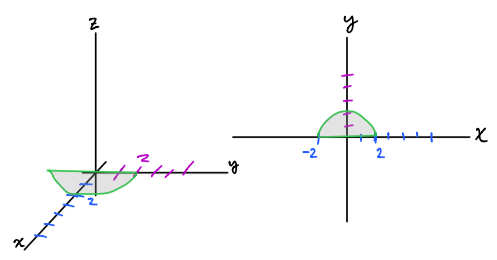
\includegraphics[width=3.5in]{img/C17p10-18.png}

\vspace{2in}


\end{document}